% arguelles v2.3.0
% author: Michele Piazzai
% contact: michele.piazzai@uc3m.es
% license: MIT

% Copied from GitHub: https://github.com/piazzai/arguelles

\documentclass[aspectratio=169,compress,12pt]{beamer}

\usetheme{Arguelles}

%%%%%%%%%%%%%%%%%%%%%%%%%%%%%%%%%%%%%%%%%%%%%%%%%
%%%%%                                       %%%%%
%%%%%     LIST OF USEFUL LaTeX PACKAGES     %%%%%
%%%%%                                       %%%%%
%%%%%%%%%%%%%%%%%%%%%%%%%%%%%%%%%%%%%%%%%%%%%%%%%

% ---
% Character encoding
% ---
\usepackage[T1]{fontenc}
\usepackage[utf8]{inputenc}
\usepackage[]{fontawesome5}

% ---
% Language related packages
% ---
\usepackage[english]{babel}
\usepackage[abbreviations,british]{foreign}

% ---
% Bibliography-related
% ---
% \usepackage[numbers, sort&compress]{natbib}
%
% ---
% Colours
% ---
\usepackage[]{color}
\usepackage[]{xcolor}

% ---
% Figures
% ---
\usepackage[]{graphicx}
\usepackage[]{subfigure}

% ---
% Mathematics
% ---
\usepackage[]{mathtools}
\usepackage[]{amssymb, amsmath, amsfonts}
\usepackage[]{yhmath}
\usepackage[]{stmaryrd}
\usepackage[]{nicefrac}
\usepackage[]{algpseudocode}

% ---
% Physics
% ---
\usepackage[]{siunitx}
\usepackage[]{physics}

% ---
% Tikz-related
% ---
\usepackage[]{tikz}
\usetikzlibrary{arrows}
\usetikzlibrary{shapes}
\usetikzlibrary{positioning}
\usetikzlibrary{tikzmark}
\usetikzlibrary{patterns}
\usetikzlibrary{backgrounds}

% ---
% Miscellaneous
% ---
\usepackage[]{lipsum}
\usepackage[]{xparse}
\usepackage{multicol}

%%%%%%%%%%%%%%%%%%%%%%%%%%%%%%%%%%%%%%%%%%%%%%%
%%%%%                                     %%%%%
%%%%%     LIST OF COMMANDS AND MACROS     %%%%%
%%%%%                                     %%%%%
%%%%%%%%%%%%%%%%%%%%%%%%%%%%%%%%%%%%%%%%%%%%%%%

% ---
% Annotating equations using Tikz
% ---
\newcommand{\highlight}[2]{\colorbox{#1!17}{\ensuremath{\displaystyle #2}}}
\newcommand{\highlightdark}[2]{\colorbox{#1!47}{\ensuremath{\displaystyle #2}}}

% ---
% Mathematics
% ---

% Simple macros
\renewcommand{\det}[1]{\text{det}\left( #1 \right)}
\renewcommand{\trace}[1]{\text{Tr}\left( #1 \right)}
\newcommand{\Span}[1]{\text{Span}\left( #1 \right)}
\newcommand{\conj}[1]{\ensuremath{#1^*}}


% Algebra
\newcommand{\e}{\ensuremath{\mathrm{e}}}

\newcommand{\R}{\ensuremath{\mathbb{R}}}
\newcommand{\C}{\ensuremath{\mathbb{C}}}
\newcommand{\K}{\ensuremath{\mathbb{K}}}

\newcommand{\innerprod}[2]{\ensuremath{\left\langle #1 \vert #2 \right\rangle}}

% Linear algebra
\newcommand{\allones}{\ensuremath{\mathbf{1}}}
\newcommand{\allzeros}{\ensuremath{\mathbf{0}}}
\newcommand{\Gram}[1]{\ensuremath{\mathbf{#1}^H \mathbf{#1}}}
\newcommand{\inv}[1]{\ensuremath{\mathbf{#1}^{-1}}}
\newcommand{\pinv}[1]{\ensuremath{\mathbf{#1}^{\dagger}}}
\newcommand{\svd}[1]{\ensuremath{\mathbf{U}_{#1} \boldsymbol{\Sigma}_{#1} \mathbf{V}^H_{#1}}}

% Probability and statistics
\newcommand{\E}[1]{\ensuremath{\mathbb{E} \left( #1 \right)}}
\newcommand{\covmat}[1]{\ensuremath{\mathbf{C}_{\mathbf{#1}}}}

% Optimization problems
\DeclareMathOperator*{\minimize}{minimize~}
\DeclareMathOperator*{\argmin}{argmin~}

\DeclareMathOperator*{\maximize}{maximize~}
\DeclareMathOperator*{\argmax}{argmax~}

\DeclareMathOperator{\subto}{subject~to~}

% Column and row vectors.
\ExplSyntaxOn
\NewDocumentCommand{\colvec}{O{1}m}
{
  \scalebox{#1}{$\generalvec{#2}{\\}$}
}
\NewDocumentCommand{\rowvec}{O{1}m}
{
  \scalebox{#1}{$\generalvec{#2}{&}$}
}
\NewDocumentCommand{\generalvec}{mm}
{
  \clist_set:Nn \l_tmpa_clist { #1 }
  %\renewcommand{\arraystretch}{.8}
  \begin{bmatrix}
    \clist_use:Nn \l_tmpa_clist { #2 }
  \end{bmatrix}
}
\ExplSyntaxOff
\usefonttheme{professionalfonts}

\graphicspath{{./imgs/}}

\title{SINDy}
\subtitle{A whirlwind tour of its ecosystem}
\event{}
\date{}
\author{Jean-Christophe Loiseau}
\institute{Arts \& Métiers}
\email{jean-christophe.loiseau@ensam.eu}
\homepage{loiseaujc.github.io}
\github{loiseaujc}

\begin{document}

\frame[plain]{\titlepage}

%%%%%%%%%%%%%%%%%%%%%%%%%%%%%%%%
%%%%%     INTRODUCTION     %%%%%
%%%%%%%%%%%%%%%%%%%%%%%%%%%%%%%%

% \begin{frame}[plain]
%     \vfill
%     \begin{minipage}{.38\textwidth}
%         \centering
%         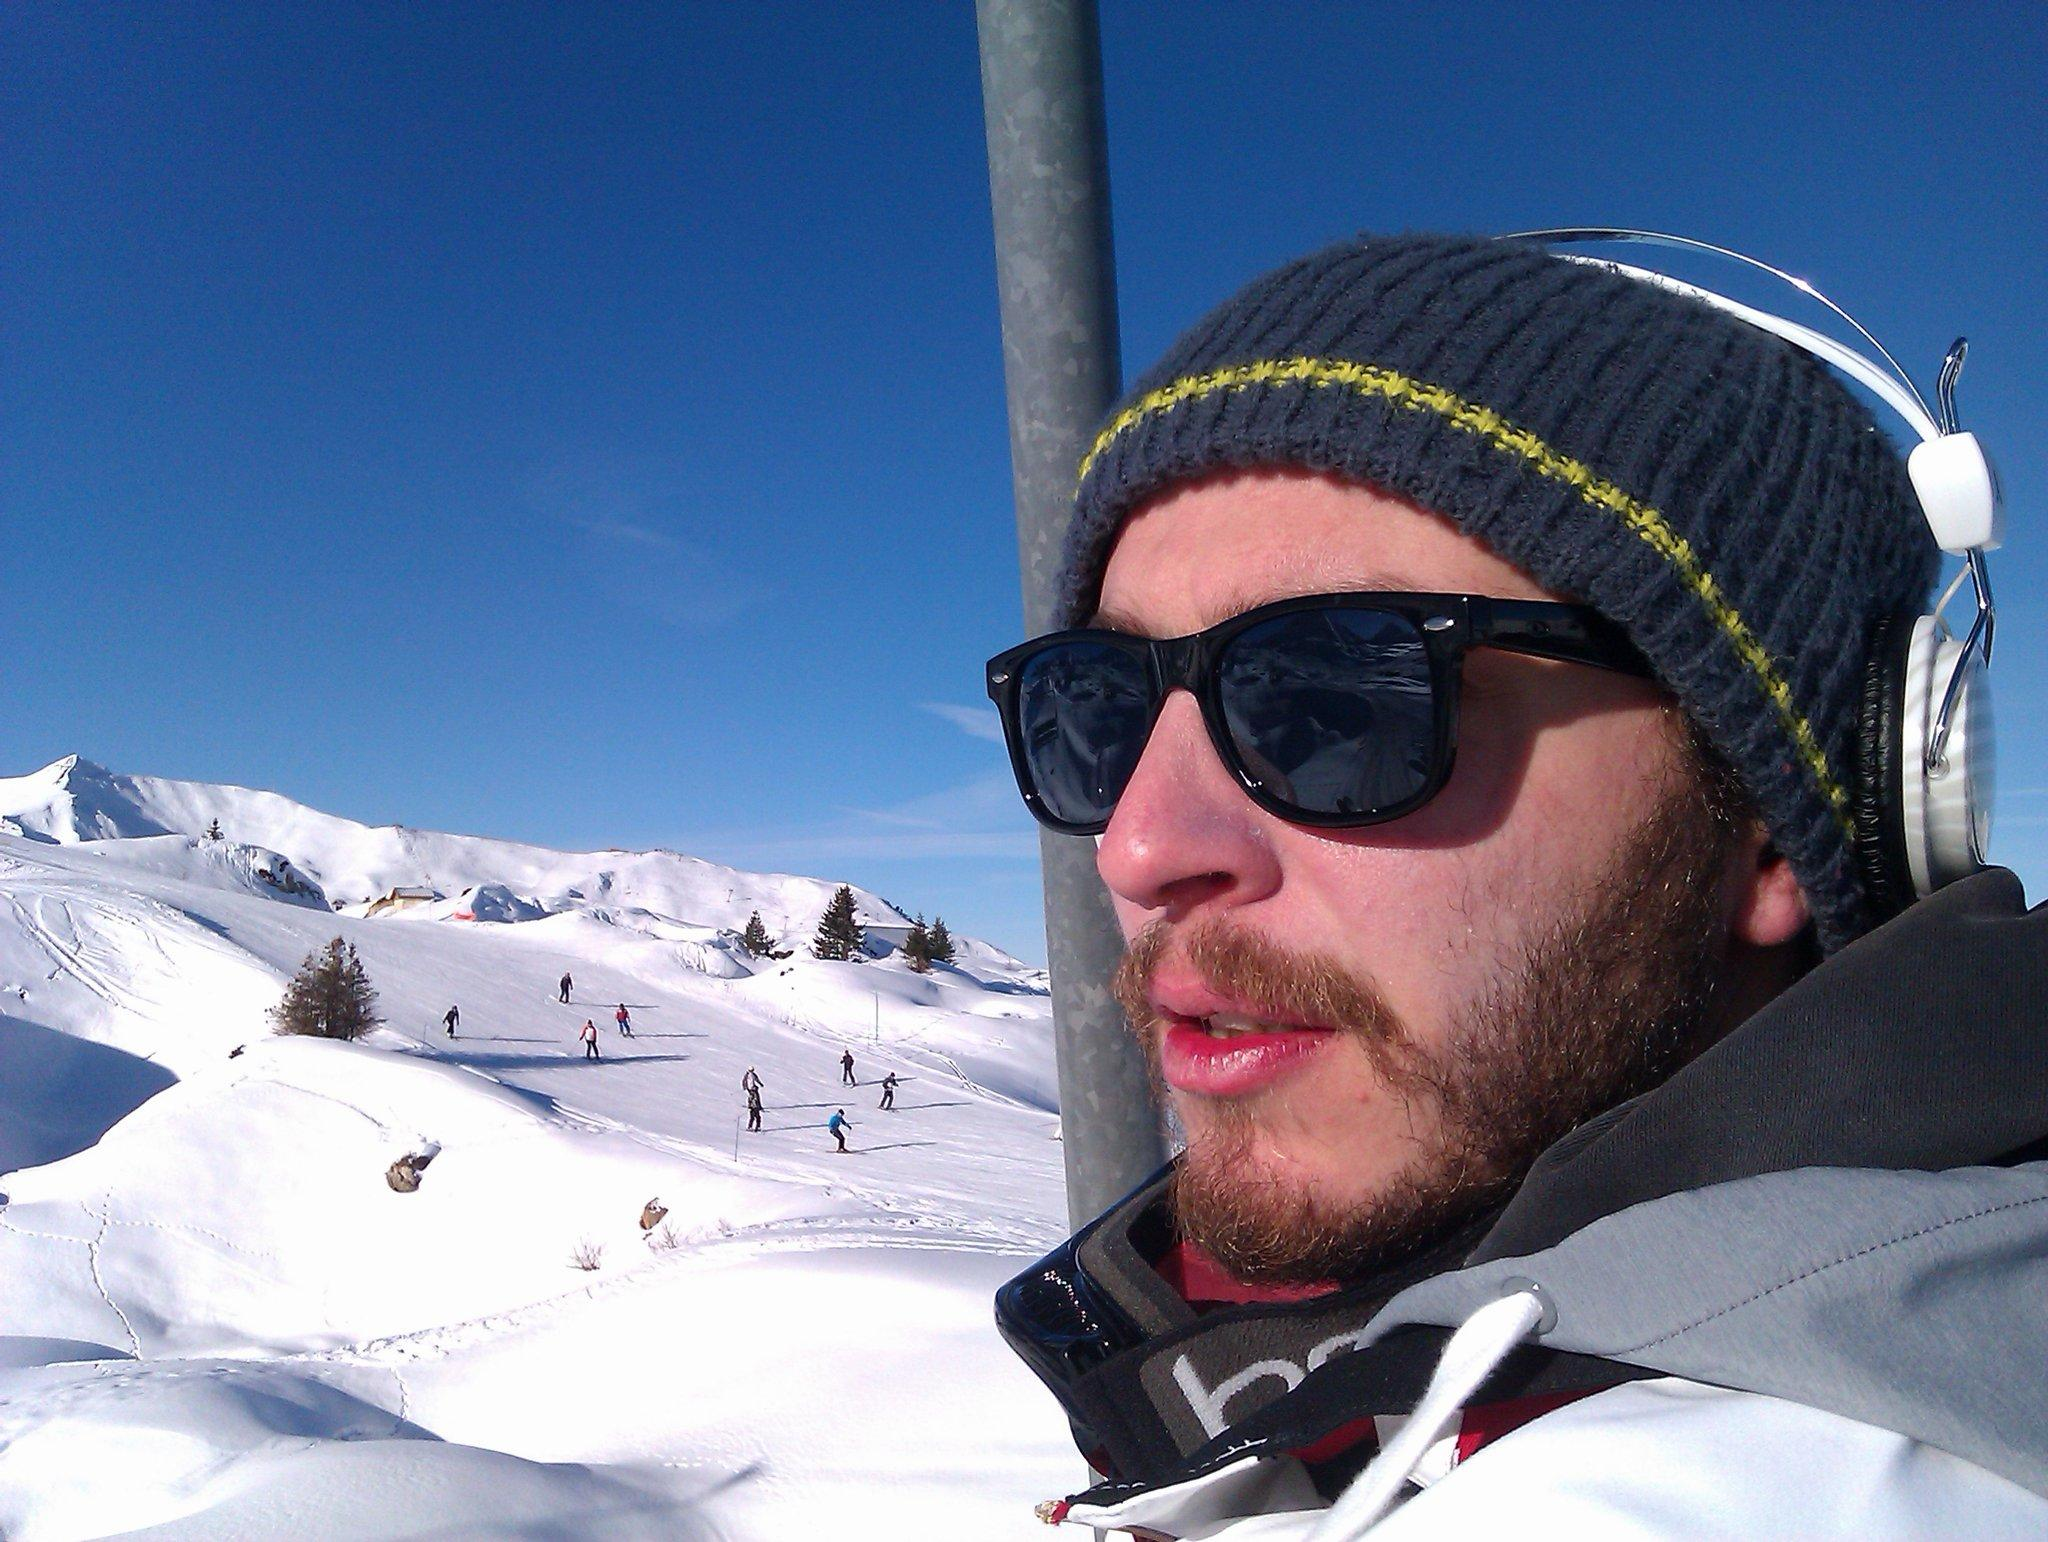
\includegraphics[width=.66\textwidth]{imgs/myself.jpg}
        
%         \bigskip
        
%         \tiny
%         Jean-Christophe Loiseau
%     \end{minipage}%
%     \hfill
%     \begin{minipage}{.58\textwidth}
%         \begin{itemize}
%             \item Assistant Prof. at ENSAM Paris

%             \medskip

%             \item Research in fluid dynamics:
%             \begin{itemize}
%                 \item Large-scale bifurcation analysis
%                 \item Stability and transition to turbulence
%                 \item ROM and sys. identification
%                 \item Flow control
%             \end{itemize}

%             \item First time ever @ CANUM !
%         \end{itemize}
%     \end{minipage}
%     \vfill
% \end{frame}

\Section{Introduction}

\begin{frame}
    \frametitle{What is SINDy?}
    \begin{minipage}{.28\textwidth}
        \centering
        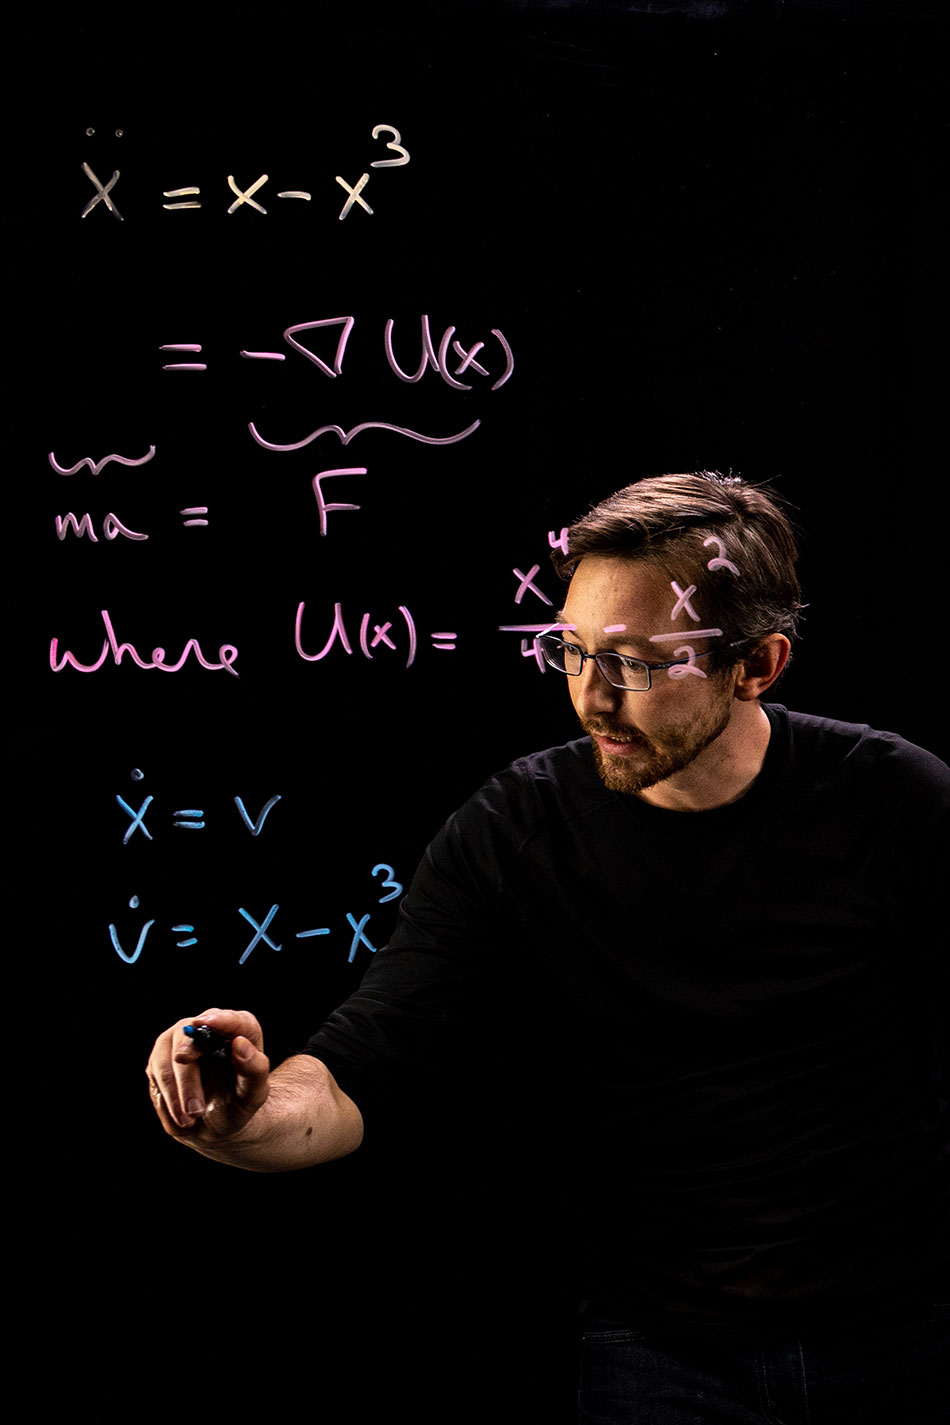
\includegraphics[width=\textwidth]{imgs/steve.jpg}
        \tiny
        Steven Brunton (UW, USA)
    \end{minipage}%
    \hfill
    \begin{minipage}{.68\textwidth}
        \vspace{-2em}
        \begin{itemize}
            \item Stands for \emph{Sparse Identification of Nonlinear Dynamics}.
            \item First paper published in 2015 in PNAS.
            \item Framework for identifying equations from data leveraging \emph{sparse regression} algorithms.
            \item Developed into a complete ecosystem since the seminal work of Steve.
        \end{itemize}
    \end{minipage}
    \vfill
\end{frame}

\begin{frame}[plain]
    \vfill
    \begin{minipage}{.68\textwidth}
        \textbf{Observation} -- Using suitable coordinates, many systems in the physical sciences are described by a set of \textbf{sparse} equations.
    \end{minipage}%
    \hfill
    \begin{minipage}{.28\textwidth}
        \centering
        \begin{overprint}
            \onslide<1>
            
\includegraphics[width=\textwidth]{imgs/ptolemaic_system.png}
            \onslide<2>
            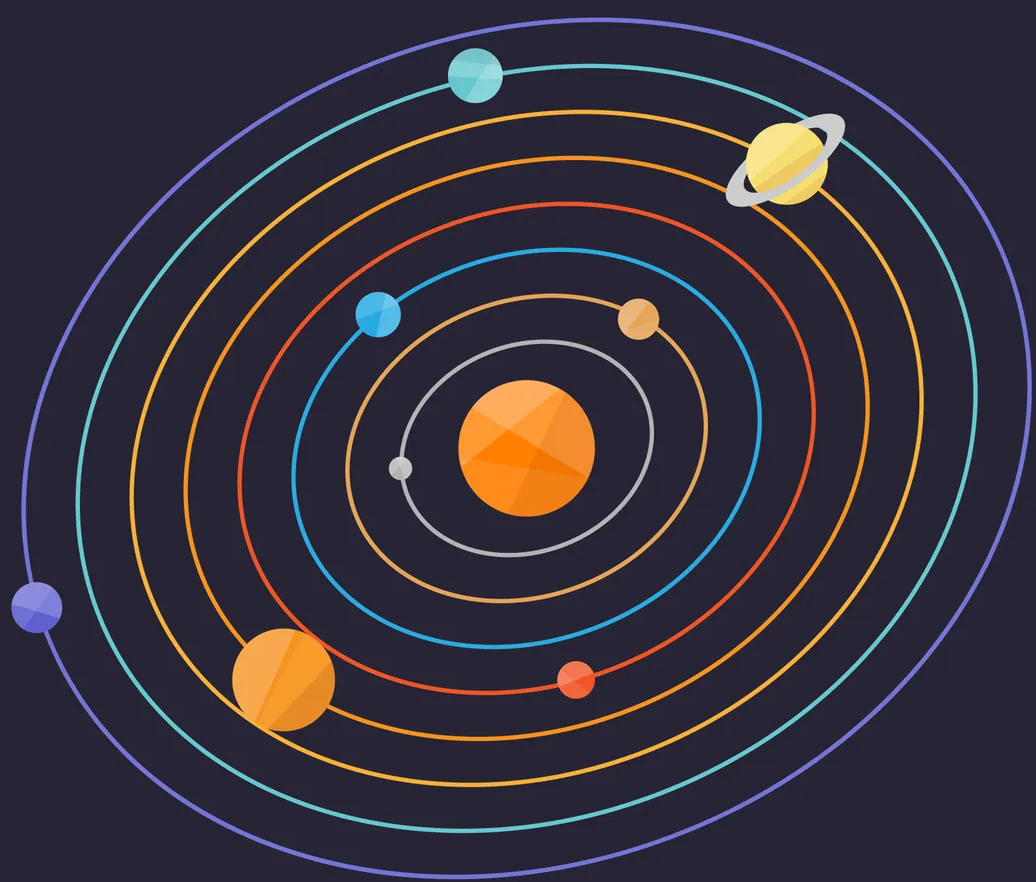
\includegraphics[width=\textwidth]{imgs/solar_system.png}
        \end{overprint}
    \end{minipage}
    \vfill
\end{frame}

\begin{frame}[plain]
    \vfill
    \centering
    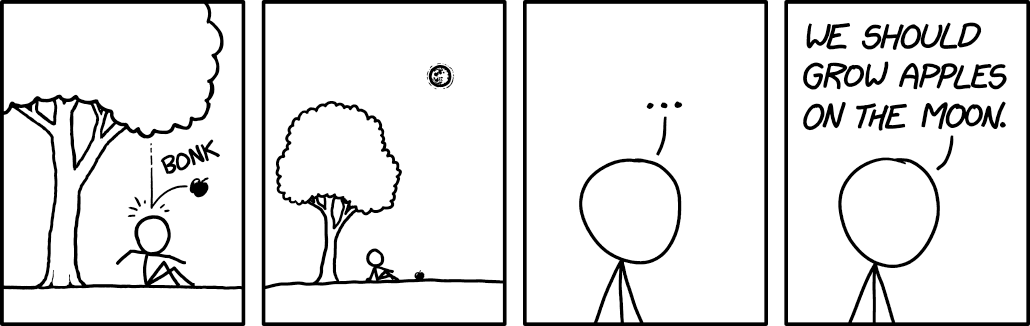
\includegraphics[width=.8\textwidth]{imgs/newton.png}
    \vfill
\end{frame}

\begin{frame}[standout, plain]
	\vfill
        \small
        \begin{multicols}{2}
            \begin{itemize}
                \item Vanilla SINDy
                \item Constrained SINDy
                \item Weak SINDy
                \item Ensemble SINDy
                \item SINDy for control
                \item SINDy-MPC
                \item SINDy-PI
                \item MANDy
                \item Langevin Regression
                \item Bayesian SINDy
                \item CINDy
                \item \ldots
            \end{itemize}
            \end{multicols}
    	\vfill
\end{frame}

\begin{frame}[standout, plain]
    \vfill
    \centering
    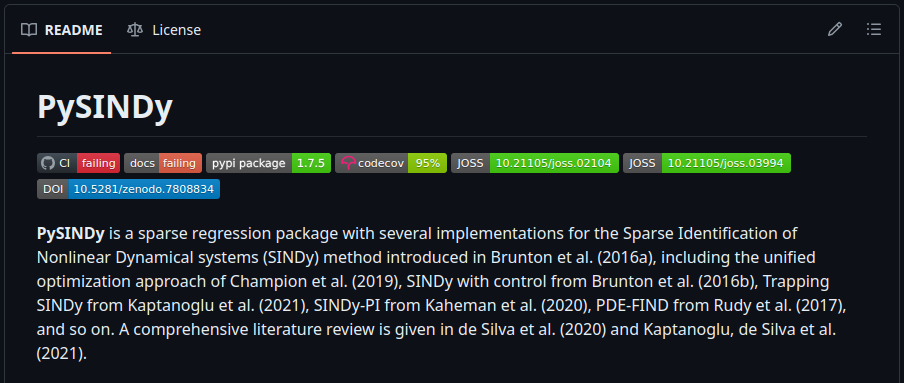
\includegraphics[width=.8\textwidth]{imgs/pysindy.png}
    \vfill
\end{frame}

\Section{SINDy for ODE}
\begin{frame}
    \frametitle{SINDy for Ordinary Diff. Eq.}
    \vfill
    \centering
    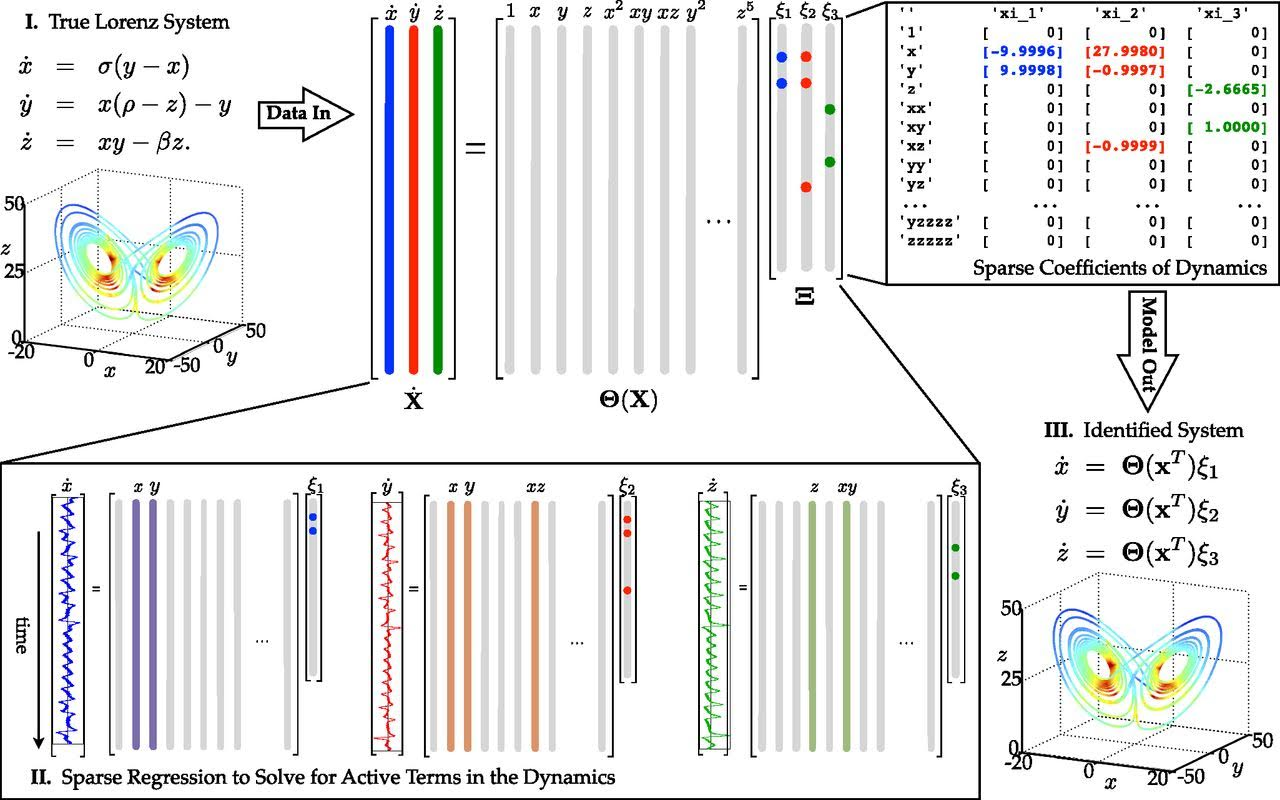
\includegraphics[height=.8\textheight]{imgs/sindy_paper.png}
    \vfill
\end{frame}

\begin{frame}
    \vfill
    \[
    \begin{aligned}
        \minimize_{\boldsymbol{\alpha}} & \quad \norm{\boldsymbol{\alpha}}_0                                                                 \\
        \subto                          & \int_{0}^T \left( \dot{\vb{x}} - f(\vb{x}) \right) \dd t = \allzeros \\
                                        & f(\vb{x}) - \sum_{i=1}^n \vartheta_i(\vb{x}) \alpha_i = \allzeros, \\
                                        & h(\vb{x}, \boldsymbol{\alpha}) = \allzeros \\
                                        & g(\vb{x}, \boldsymbol{\alpha}) \preccurlyeq \allzeros.
    \end{aligned}
    \]
    \vfill
\end{frame}

\begin{frame}
    \vfill
    \[
    \begin{aligned}
        \minimize_{\boldsymbol{\alpha}} & \quad \norm{\boldsymbol{\alpha}}_1 \\
        \subto                          & \norm{\dot{\vb{X}} - \boldsymbol{\Theta}(\vb{X}) \boldsymbol{\alpha}}_F^2 \leq \varepsilon \\
                                        & h(\vb{x}, \boldsymbol{\alpha}) = \allzeros                                                         \\
                                        & g(\vb{x}, \boldsymbol{\alpha}) \preccurlyeq \allzeros.
    \end{aligned}
    \]
    \vfill
\end{frame}

% \begin{frame}
%     \frametitle{Sparse calibration of a POD-Galerkin ROM}
%     \vfill
%     \begin{minipage}{.28\textwidth}
%         \centering
%         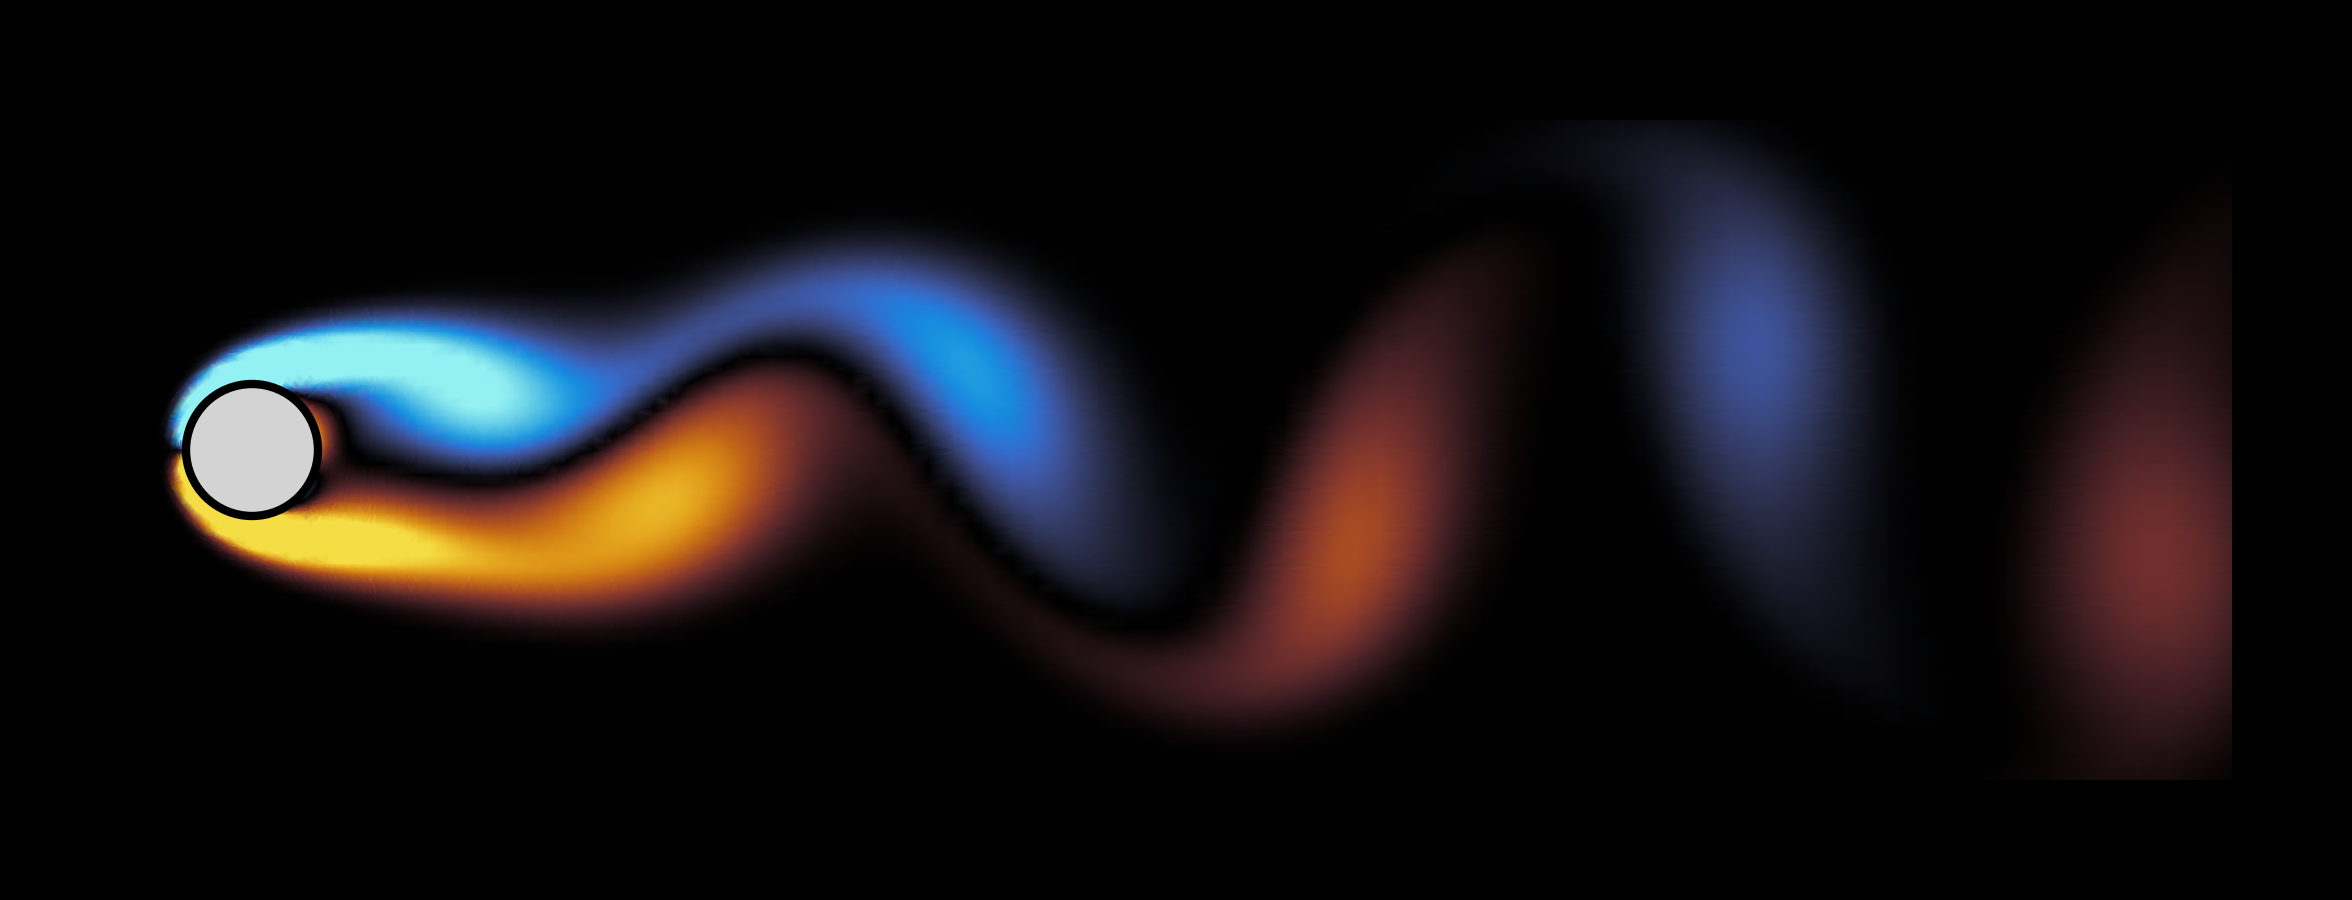
\includegraphics[height=.3\textheight, angle=-90, origin=c]{von_karman}
%     \end{minipage}%
%     \hfill
%     \begin{minipage}{.68\textwidth}
%         \centering
%         \textbf{POD-Galerkin ROM}
%         \[
%             \dot{x}_i = \sum_{j=1}^r L_{ij} x_j + \sum_{j, k=1}^r Q_{ijk} x_j x_k
%         \]
%     \end{minipage}
%     \vfill
% \end{frame}

% \begin{frame}
%     \vfill
%     \begin{minipage}{.48\textwidth}
%         \centering
%         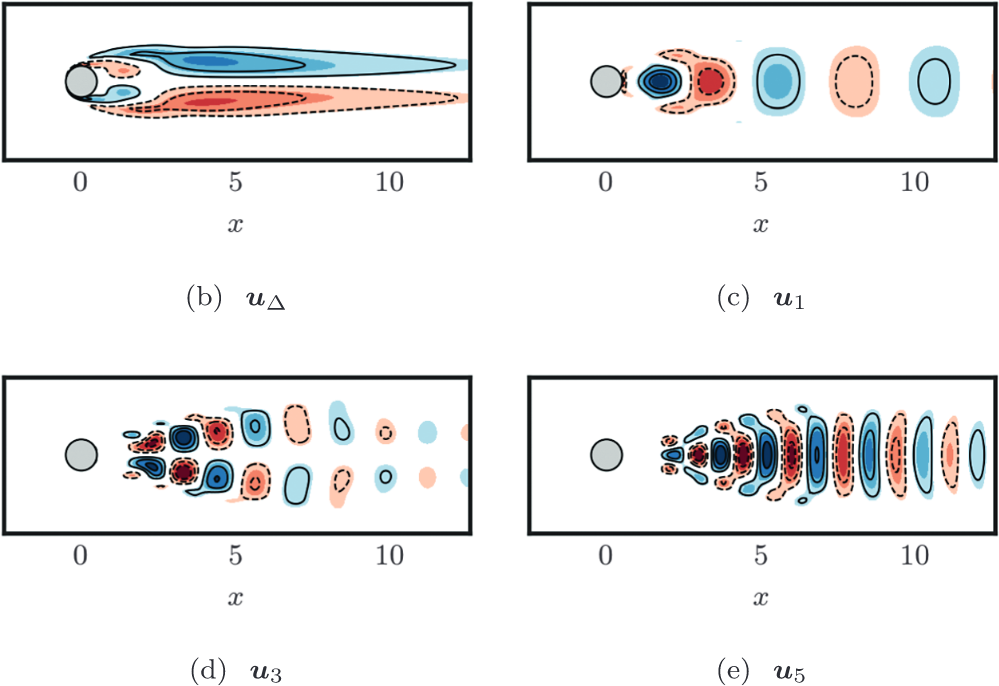
\includegraphics[width=\textwidth]{imgs/pod_cylinder.png}
%     \end{minipage}%
%     \hfill
%     \begin{minipage}{.48\textwidth}
%         \begin{itemize}
%             \item 3 POD modes capture 99\% of the variance.
%             \begin{itemize}
%                 \item Two for the von Kàrmàn vortex shedding.
%                 \item One for the distortion between the fixed point and the mean flow.
%             \end{itemize}
%             \par\bigskip
%             \item Yet, POD-Galerkin projection ROM has very limited accuracy.
%         \end{itemize}
%     \end{minipage}
%     \vfill
% \end{frame}

% \begin{frame}
%     \vfill
%     \centering
%     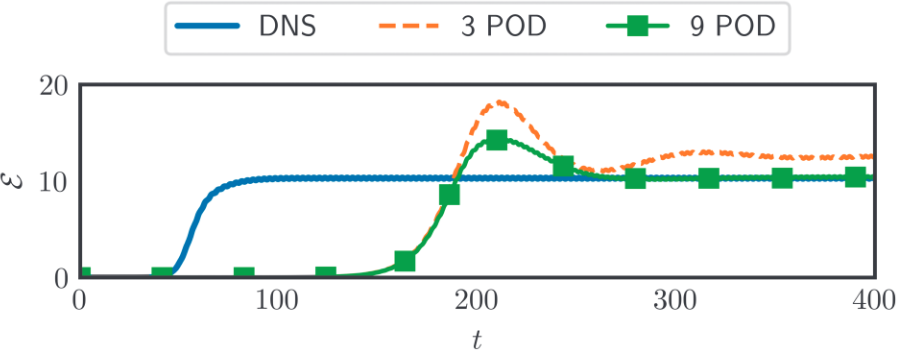
\includegraphics[width=\textwidth]{imgs/pod_galerkin_tke_cylinder.png}
%     \vfill
% \end{frame}

% \begin{frame}
%     \vfill
%     \centering
%     \textbf{"Normal form" POD-Galerkin ROM}
%     \bigskip
%     \[
%     \dot{x}_i = \sum_{j} L_{ij} x_j + \sum_{j, k} Q_{ijk} x_j x_k + \sum_{j, k, l} C_{ijkl} x_j x_k x_l
%     \]
%     \vfill
% \end{frame}

% \begin{frame}
%     \vfill
%     \begin{minipage}{.68\textwidth}
%         \begin{itemize}
%             \item Based from first principles and symmetry considerations:
%             %
%             \begin{itemize}
%                 \item $L_{ij} = \vb{u}_i^T \vb{A} \vb{u}_j$ is block-diagonal,
%                 \item $L_{33}$ is negative,
%                 \item $Q_{ijk}$ is skew-symmetric,
%                 \item $C_{ijkl}$ is dissipative.
%             \end{itemize}
%             \item All these lead to linear equality or inequality constraints.
%         \end{itemize}
%     \end{minipage}%
%     \hfill
%     \begin{minipage}{.28\textwidth}
    
%     \end{minipage}
%     \vfill
% \end{frame}

% \begin{frame}
%     \vfill
%     \[
%     \begin{aligned}
%         \minimize_{\bf{L}, \vb{Q}, \bf{C}} & \quad \norm{\bf{L}}_0 + \norm{\vb{Q}}_0 + \norm{\vb{C}}_0 \\
%         \subto                          & \norm{\dot{x}_i - L_{ij}x_j - Q_{ijk} x_j x_k - C_{ijkl} x_j x_k x_l }^2 \leq \varepsilon \\
%                                         & L_{1, 2} =  L_{1, 3} = 0, \\
%                                         & L_{2, 2} =  L_{2, 3} = 0, \\
%                                         & L_{3, 1} = L_{3, 2} = 0, \\
%                                         & L_{3, 3} \leq 0, \\
%                                         & Q_{iii} = Q_{ijk} - Q_{ikj} = 0, \\
%                                         & g(\vb{C}) \preccurlyeq \allzeros.
%     \end{aligned}
%     \]
%     \vfill
% \end{frame}

% \begin{frame}
%     \vfill
%     \centering
%     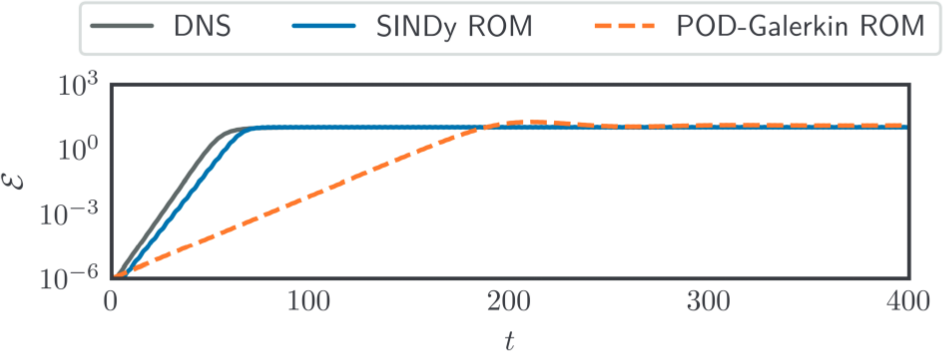
\includegraphics[width=\textwidth]{imgs/sindy_galerkin_tke_cylinder.png}
%     \vfill
% \end{frame}

% \begin{frame}
%     \vfill
%     \centering
%     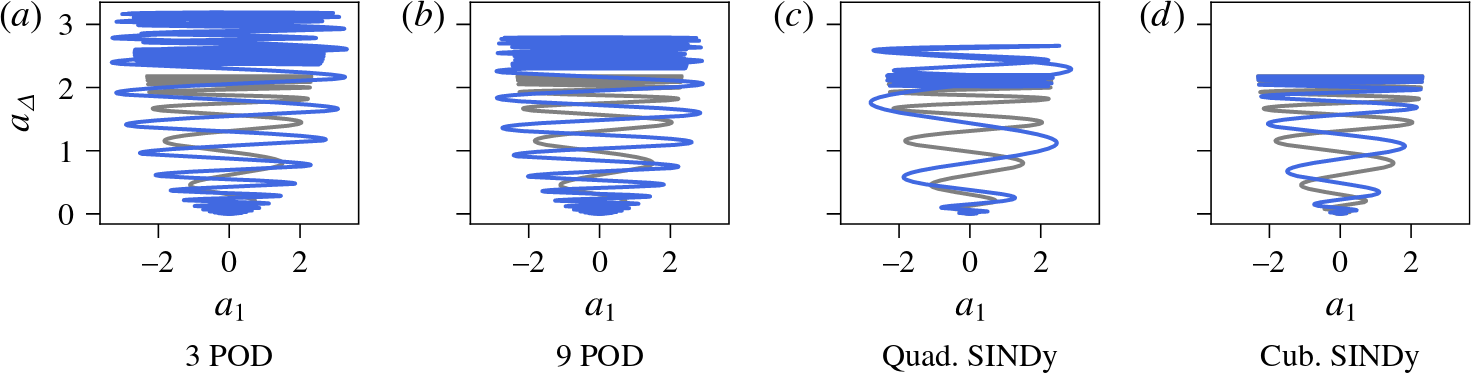
\includegraphics[width=\textwidth]{imgs/cylinder_attractor.png}
%     \vfill
% \end{frame}

\begin{frame}
    \frametitle{Identifying normal forms}
    \vfill
    \begin{minipage}{.38\textwidth}
        \centering
        
\includegraphics[width=\textwidth]{imgs/cavity_geomtry.png}
    \end{minipage}%
    \hfill
    \begin{minipage}{.58\textwidth}
        \begin{itemize}
            \item Classical example in flow control.
            \par\bigskip
            \item At $Re = 7500$, the dynamics are \emph{quasiperiodic}.
            \par\bigskip
            \item 64 POD modes required to capture 99\% of the fluctuations.
        \end{itemize}
    \end{minipage}
    \vfill
\end{frame}

\begin{frame}
    \vfill
    \centering
    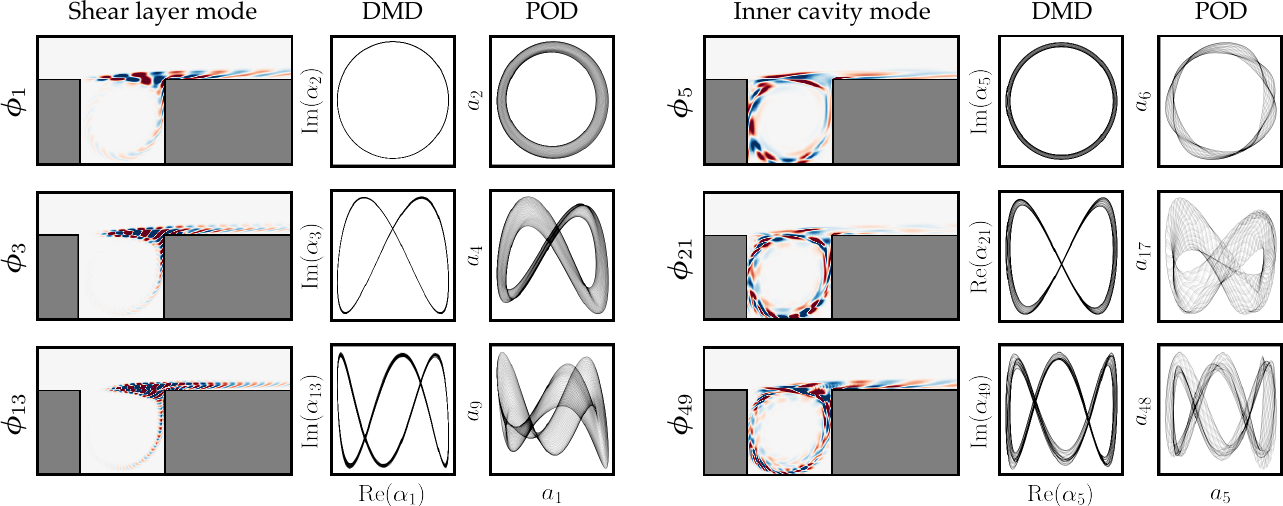
\includegraphics[width=\textwidth]{imgs/pod_modes.png}
    \vfill
\end{frame}

\begin{frame}
    \vfill
    \centering
    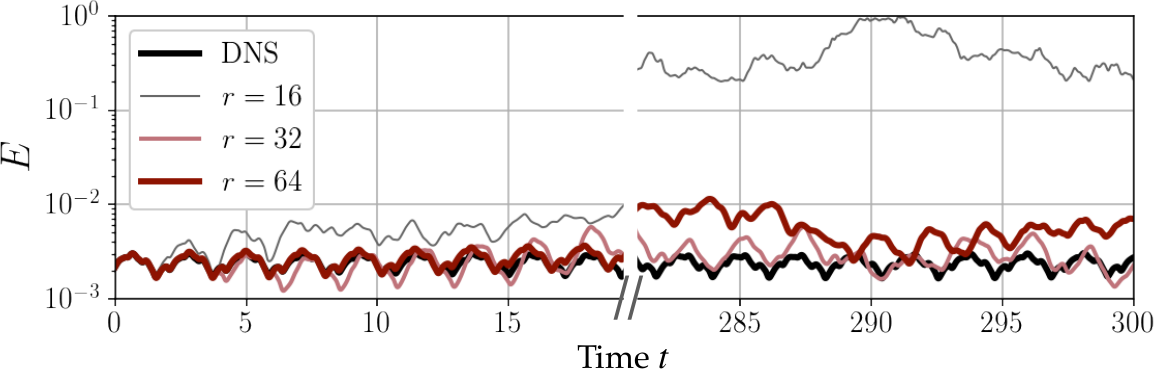
\includegraphics[width=\textwidth]{imgs/tke_galerkin.png}
    \vfill
\end{frame}

\begin{frame}
    \vfill
    \begin{minipage}{.48\textwidth}
        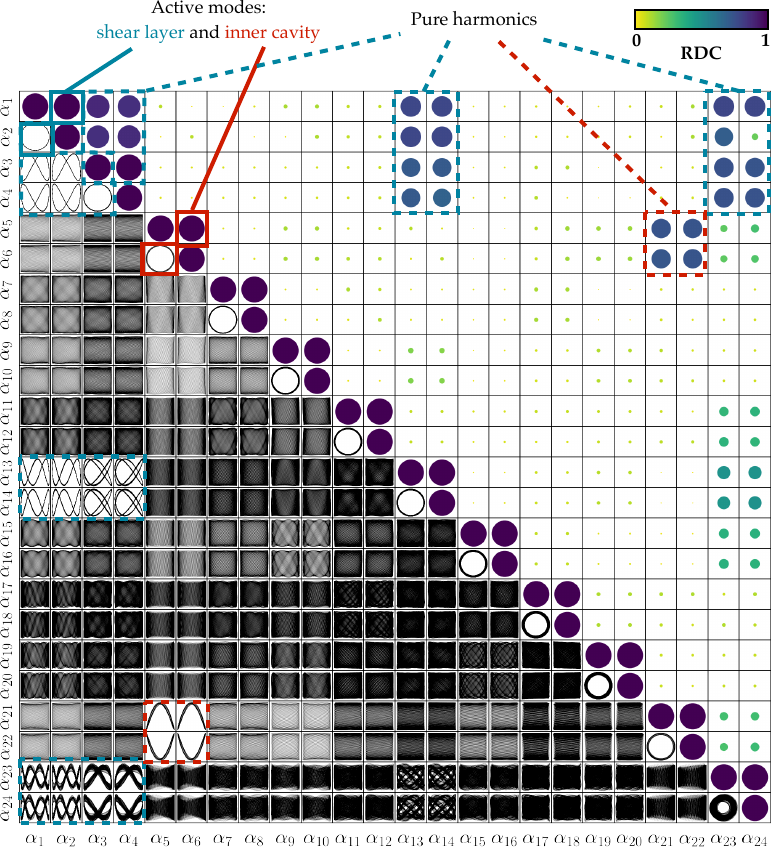
\includegraphics[width=\textwidth]{imgs/rdc_score.png}
    \end{minipage}%
    \hfill
    \begin{minipage}{.48\textwidth}
        \begin{itemize}
            \item Many modes are artifacts coming from representing a low-dimensional manifold in a large Euclidean space.
            \par\bigskip
            \item Need to find a way to break the \emph{Kolmogorov n-width}.
        \end{itemize}
    \end{minipage}
    \vfill
\end{frame}

\begin{frame}
    \vfill
    \begin{minipage}{.48\textwidth}
        \begin{itemize}
            \item Using only the four active degrees of freedom, SINDy identifies
            %
            \[
            \begin{aligned}
                \dot{x} & = \lambda_1 x - \mu_1 \abs{x}^2 x \\
                \dot{y} & = \lambda_2 y - \mu_2 \abs{y}^2 y.
            \end{aligned}
            \]
            \item ROM consistent with the known bifurcation diagram of the problem.
        \end{itemize}
    \end{minipage}%
    \hfill
    \begin{minipage}{.48\textwidth}
        \centering
        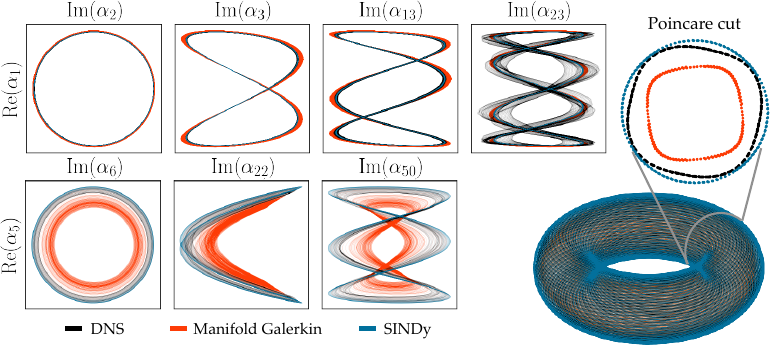
\includegraphics[width=\textwidth]{imgs/sindy_attractor.png}
    \end{minipage}
    \vfill
\end{frame}

\begin{frame}
    \vfill
    \centering
    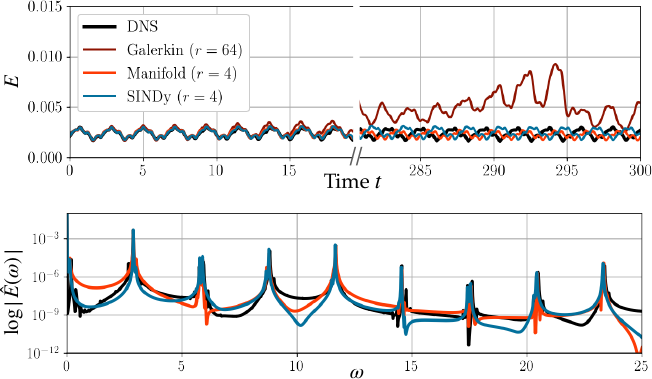
\includegraphics[width=.8\textwidth]{imgs/sindy_tke.png}
    \vfill
\end{frame}

\Section{Finding PDEs}
\begin{frame}
    \frametitle{SINDy for Partial Diff. Eq.}
    \vfill
    \begin{minipage}{.28\textwidth}
        \centering
        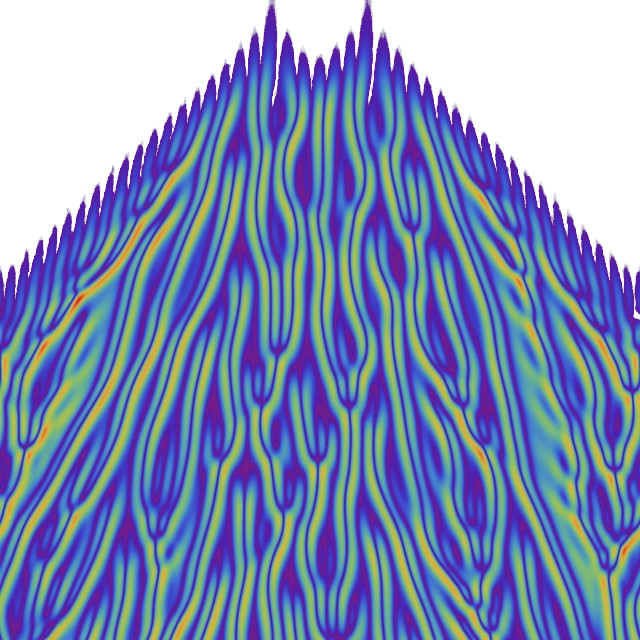
\includegraphics[width=\textwidth]{imgs/kuramoto.png}
    \end{minipage}%
    \hfill
    \begin{minipage}{.68\textwidth}
        \begin{itemize}
            \item Extending SINDy to PDE is straightforward.
            \par\bigskip
            \item Massively over-determined constrained least-squares problem.
        \end{itemize}
    \end{minipage}
    \vfill
\end{frame}

\begin{frame}
    \vfill
    \centering
    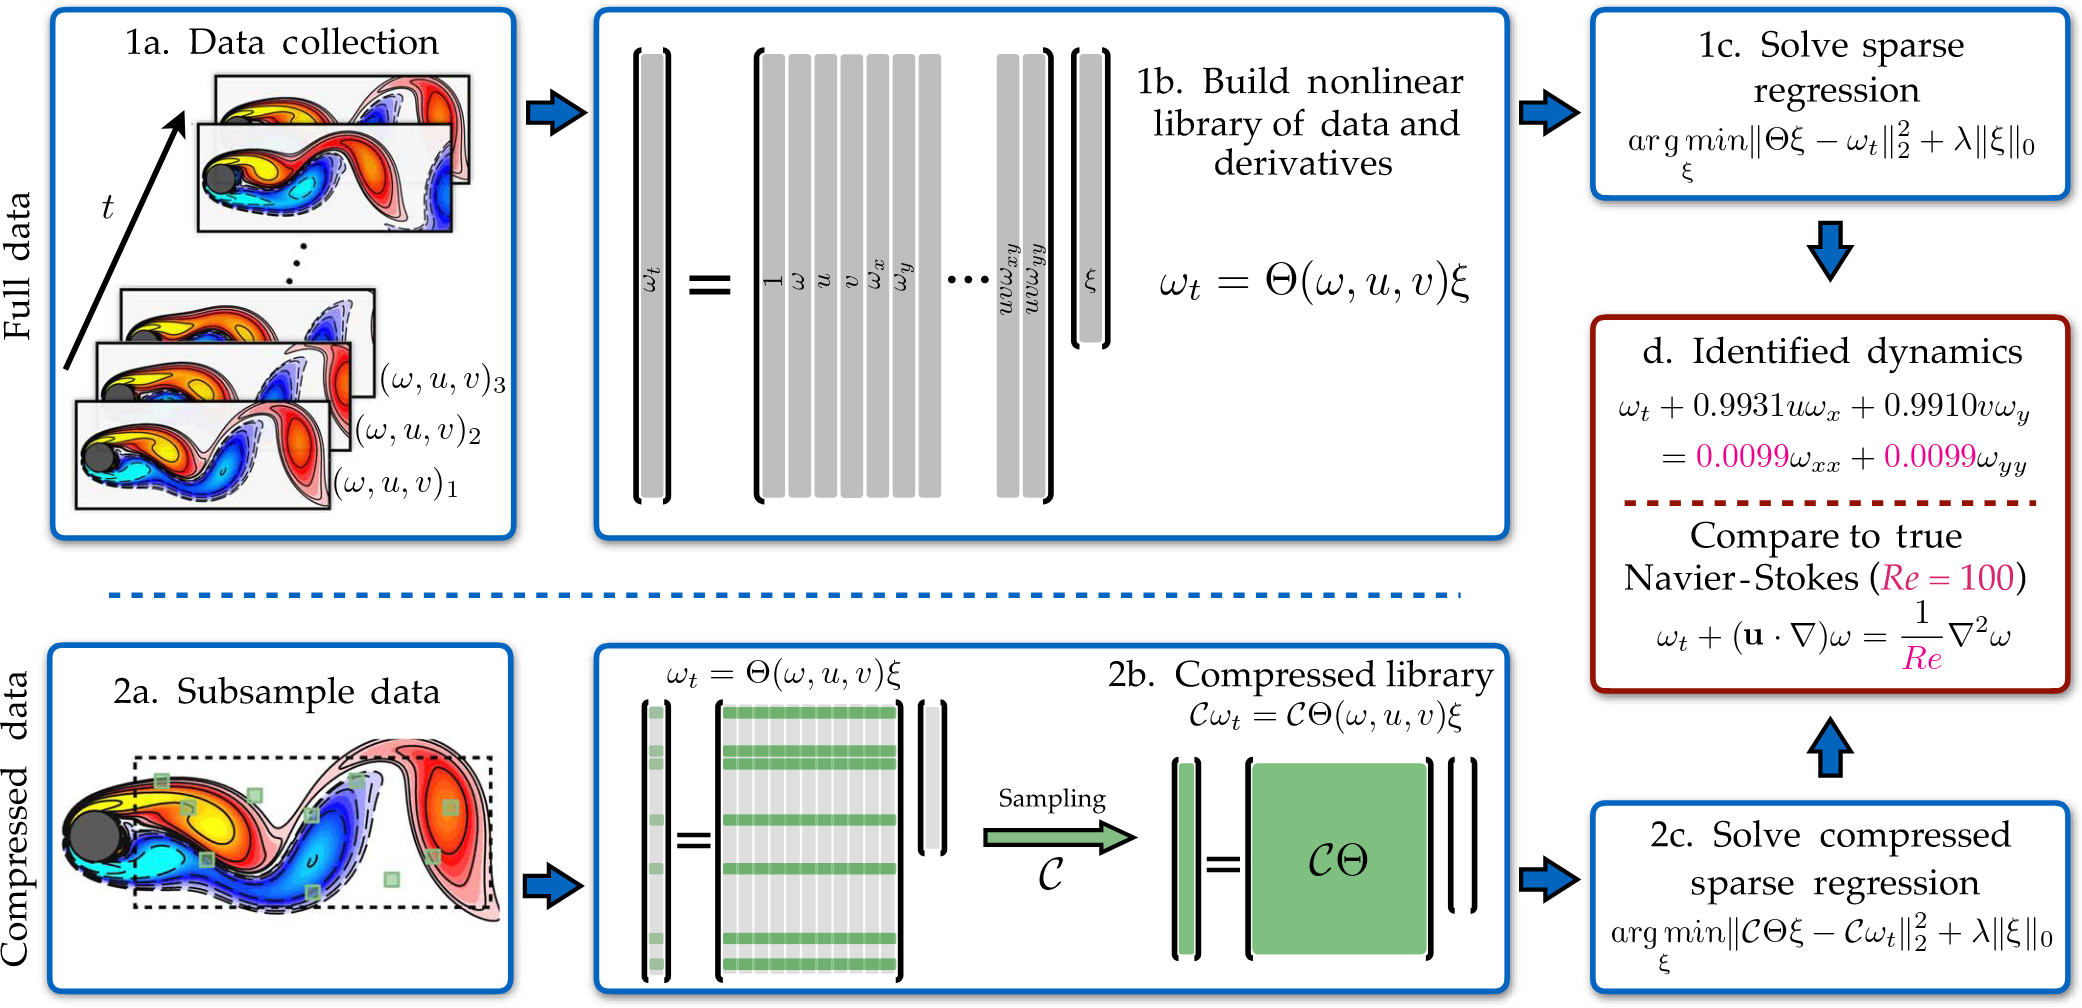
\includegraphics[width=\textwidth]{imgs/pde_find.png}
    \vfill
\end{frame}

\begin{frame}[plain, standout]
    \vfill
    \centering
    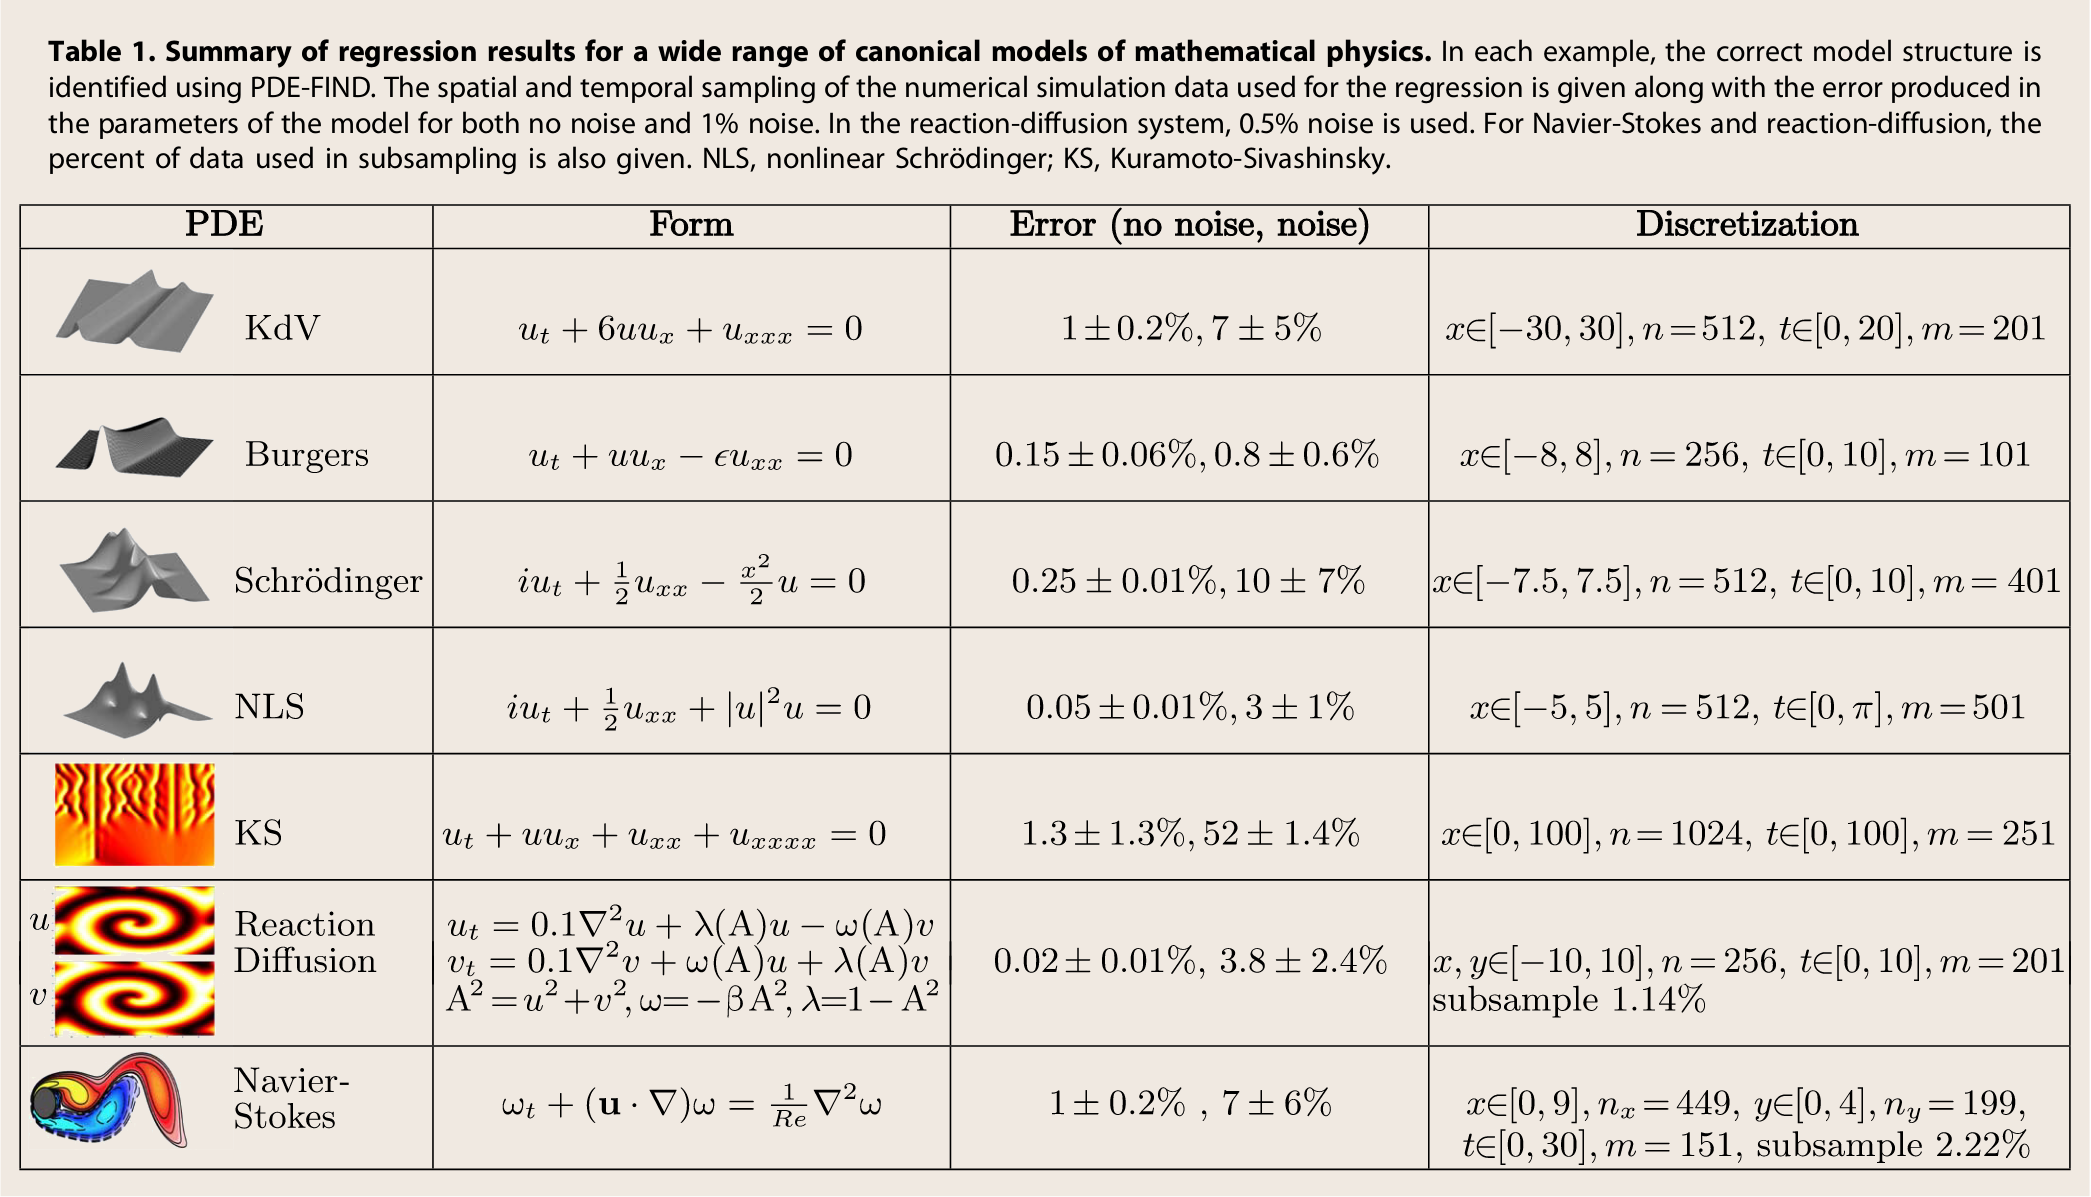
\includegraphics[width=\textwidth]{imgs/pde_find_results.png}
    \vfill
\end{frame}

\begin{frame}
    \vfill
    \begin{minipage}{.68\textwidth}
        \begin{itemize}
            \item Physical assumptions of \emph{smoothness}, \emph{locality} and \emph{symmetry} can be used to design an admissible dictionary.
            \par\bigskip
            \item Currently being used at CEA to infer a PDE from experimental PIV measurements of active turbulence.
            \par\bigskip
            \item Recent extension of incorporate assumptions of \emph{smoothness}, \emph{locality} and \emph{symmetry} to design \emph{a priori} a physically admissible dictionary.
        \end{itemize}
    \end{minipage}%
    \hfill
    \begin{minipage}{.28\textwidth}
        \centering
        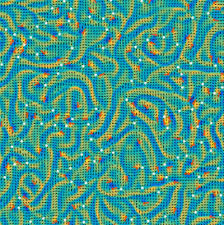
\includegraphics[width=\textwidth]{imgs/active_turbulence.jpeg}
    \end{minipage}
    \vfill
\end{frame}

\Section{SINDy for SDE}
\begin{frame}
    \frametitle{SINDy for Stochastic Diff. Eq.}
    \vfill
    \begin{minipage}{.48\textwidth}
        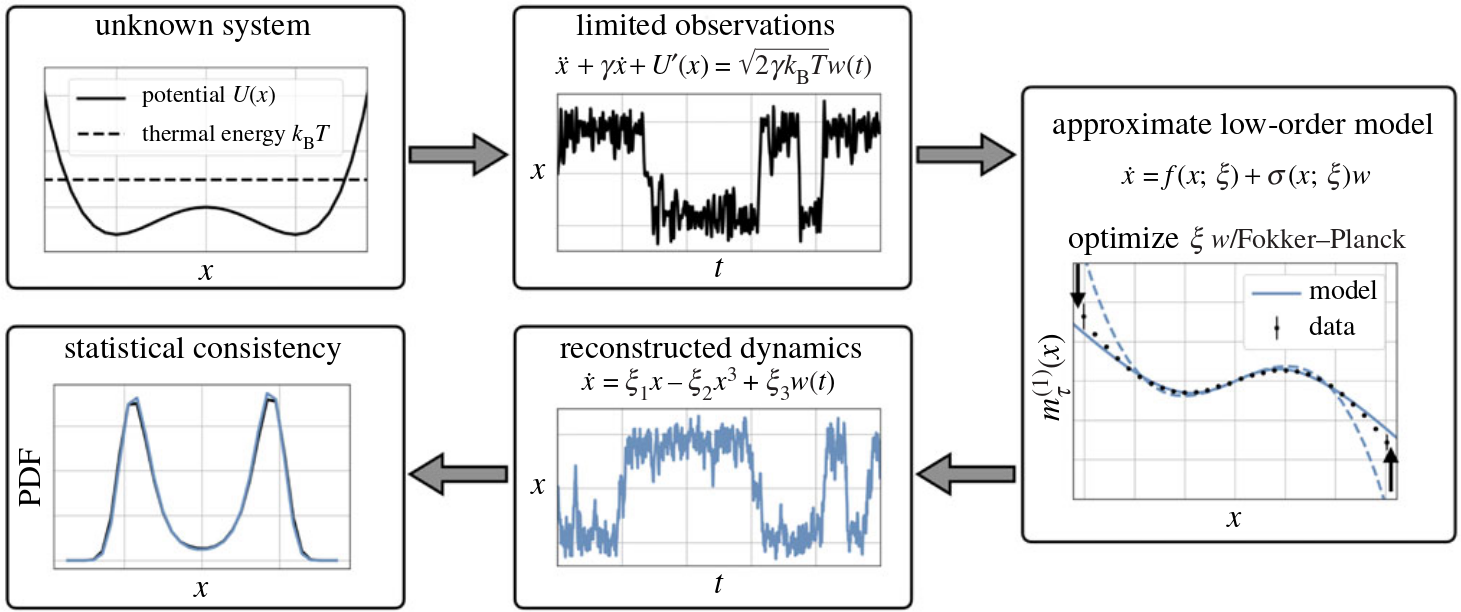
\includegraphics[width=\textwidth]{imgs/langevin_regression_one.png}
    \end{minipage}%
    \hfill
    \begin{minipage}{.48\textwidth}
        \begin{itemize}
            \item Many systems in physics can be described by \emph{Langevin equations}
            %
            \[
            \dot{x} = f(x) + \sigma(x) \eta.
            \]
            \item Identifying the drift and diffusion terms are is slightly more involved than vanilla SINDy.
        \end{itemize}
    \end{minipage}
    \vfill
\end{frame}

\begin{frame}
    \vfill
    \centering
    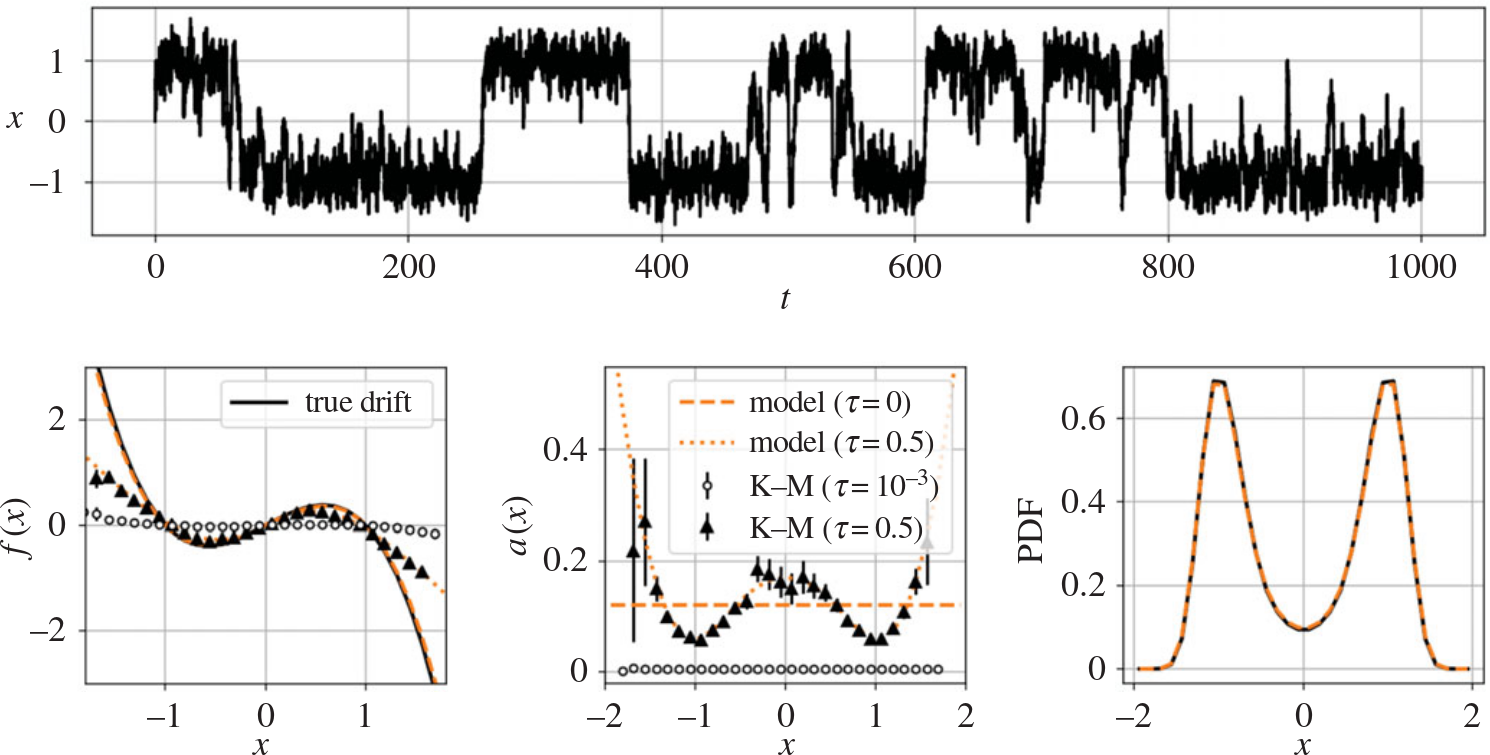
\includegraphics[width=\textwidth]{imgs/langevin_regression_three.png}
    \vfill
\end{frame}

\begin{frame}
    \vfill
    \centering
    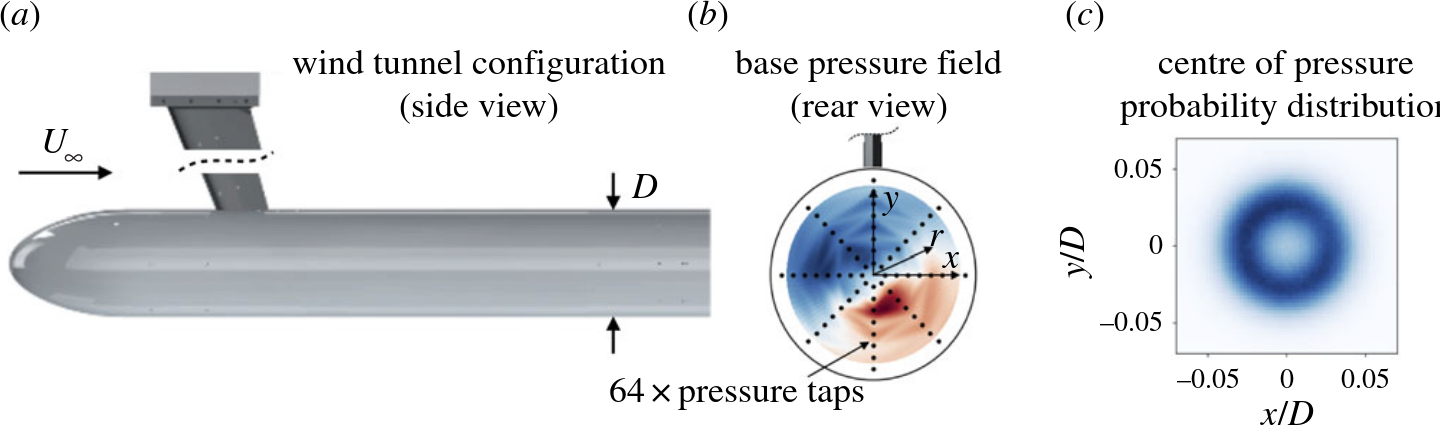
\includegraphics[width=\textwidth]{imgs/langevin_regression_four.png}
    \vfill
\end{frame}

\begin{frame}
    \vfill
    \centering
    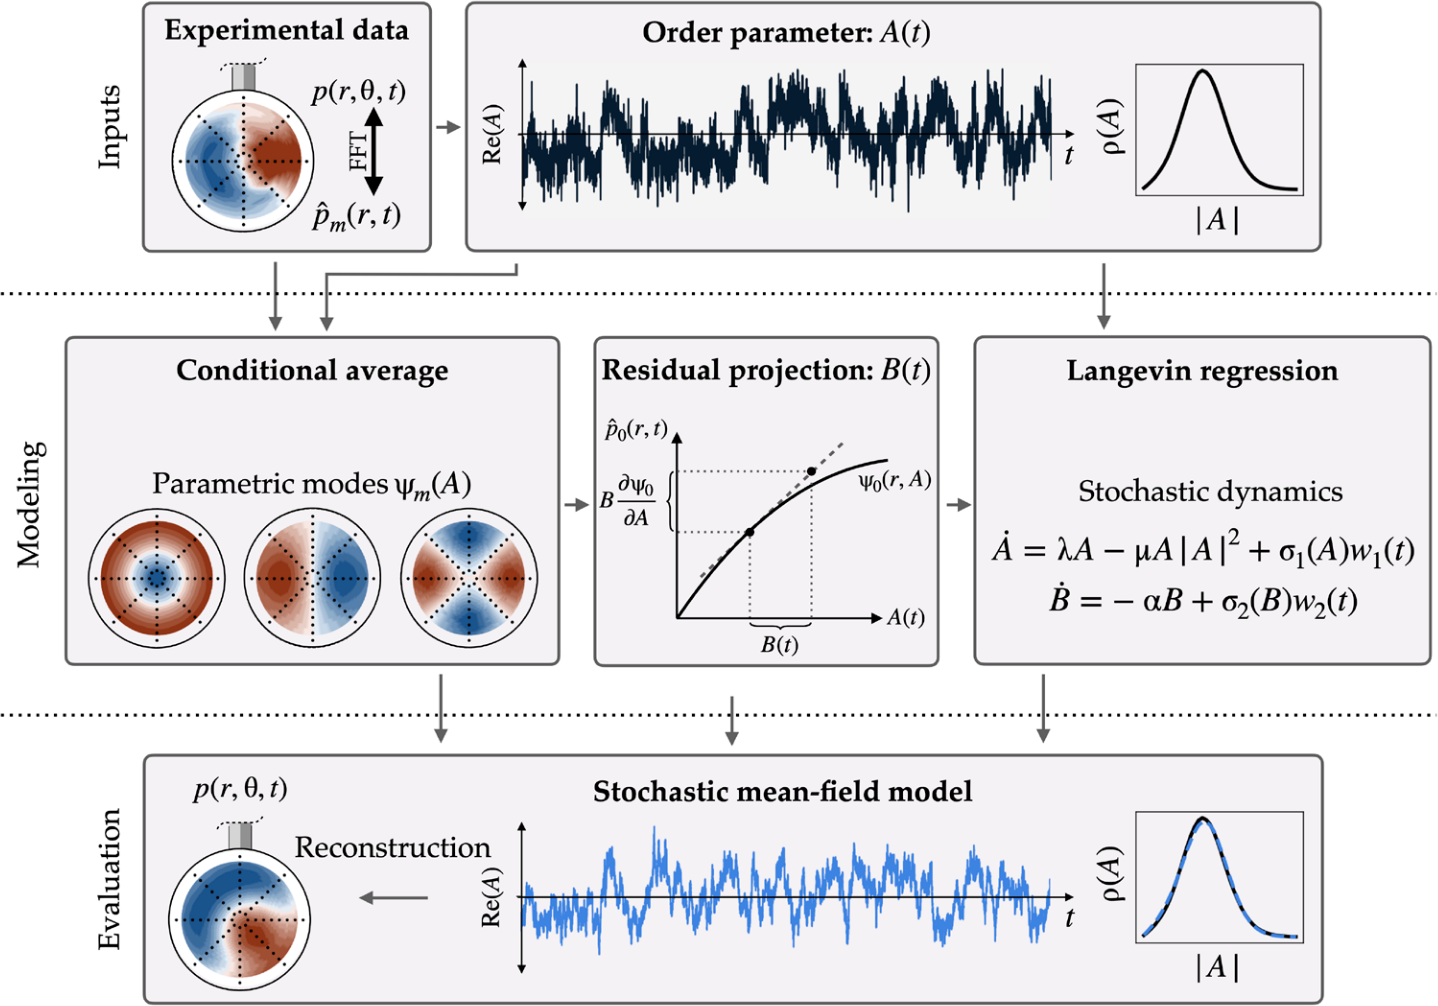
\includegraphics[height=.9\textheight]{imgs/langevin_regression_five.png}
    \vfill
\end{frame}

\Section{Reinf. Learning}
\begin{frame}
    \frametitle{SINDy for Reinf. Learning}
    \vfill
    \centering
    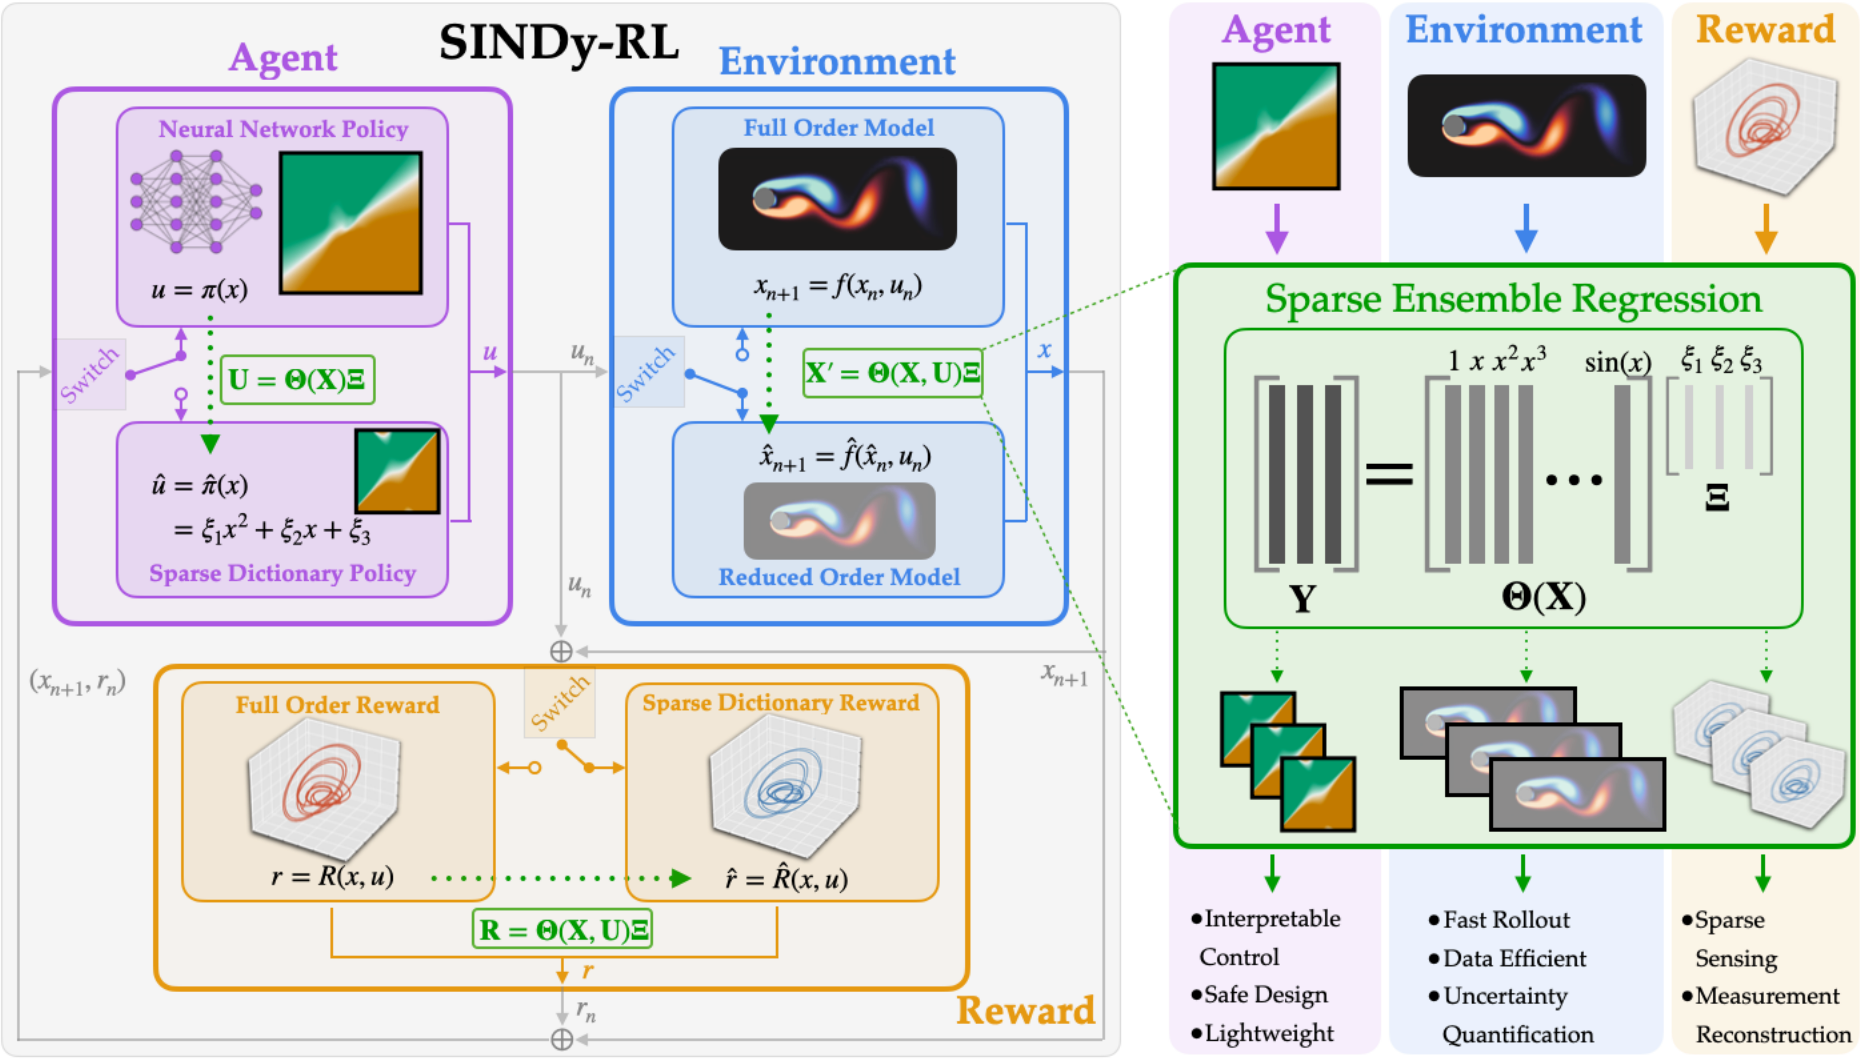
\includegraphics[width=.8\textwidth]{imgs/sindy_rl_one.png}
    \vfill
\end{frame}

\begin{frame}
    \vfill
    \centering
    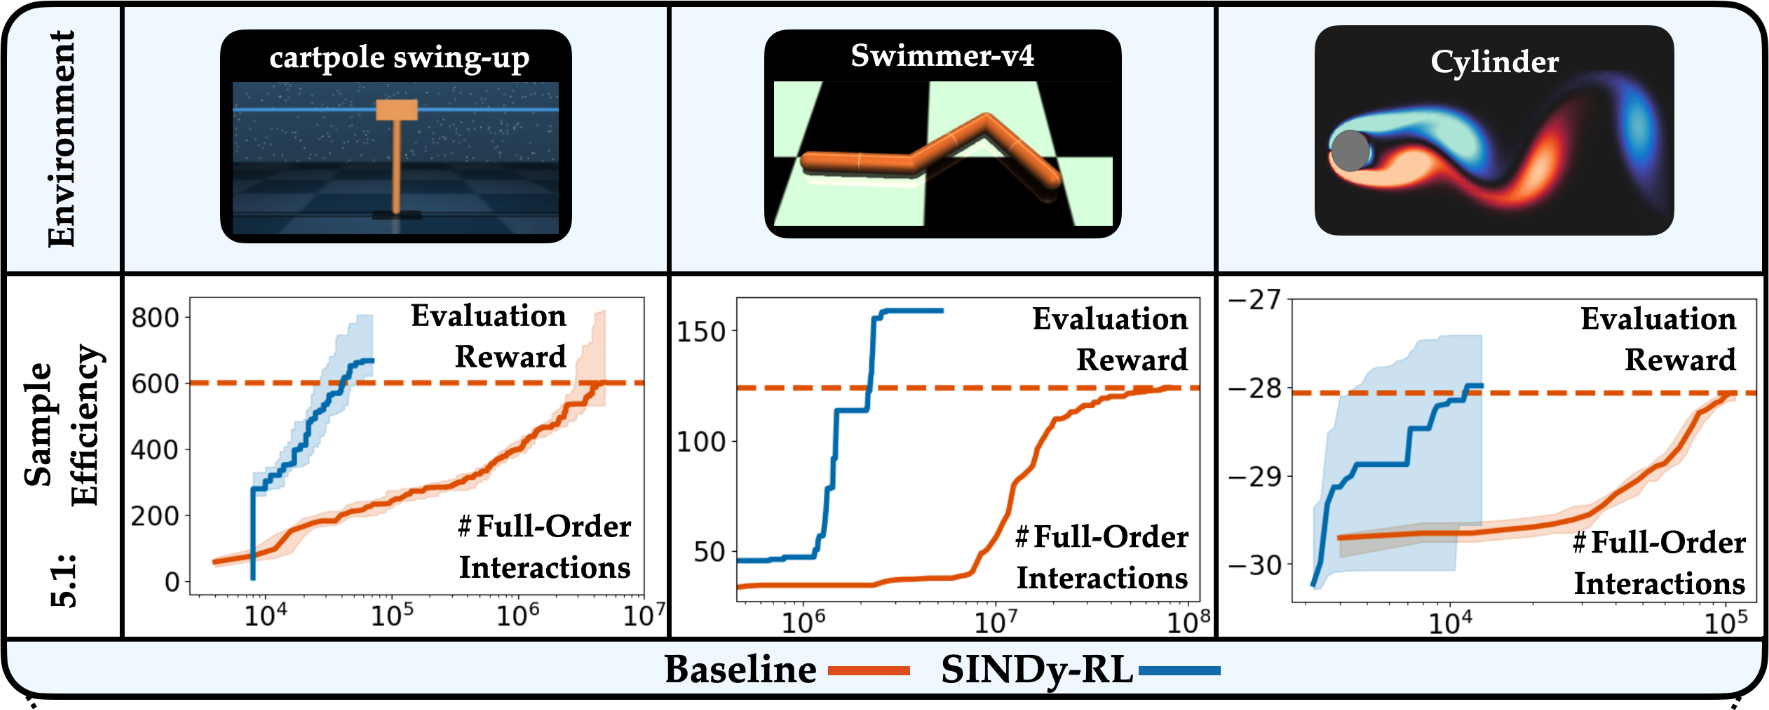
\includegraphics[width=\textwidth]{imgs/sindy_rl_two.png}
    \vfill
\end{frame}

% \Section{Control theory}
% \begin{frame}
%     \frametitle{SINDy for control systems}
% \end{frame}

\Section{Conclusion}
\begin{frame}[plain, standout]
    \vfill
    \begin{minipage}{.48\textwidth}
        \centering
        \Huge
        \textbf{Conclusion}
    \end{minipage}%
    \hfill
    \begin{minipage}{.48\textwidth}
    \end{minipage}
    \vfill
\end{frame}

\begin{frame}
    \frametitle{Conclusion}

    \vfill
    \begin{minipage}{.68\textwidth}
        \begin{itemize}
            \item Since 2015, \textbf{SINDy} has evolved into a mature ecosystem.
            \begin{itemize}
                \item Ordinary diff. eq., partial diff. eq., control systems, etc.
            \end{itemize}
            \par\bigskip
            \item Despite its versatility, \textbf{SINDy} is not a silver bullet.
            \begin{itemize}
                \item Requires quite a bit of domain expertise.
            \end{itemize}
        \end{itemize}
    \end{minipage}%
    \hfill
    \begin{minipage}{.28\textwidth}
        \centering
        
\includegraphics[width=\textwidth]{imgs/conclusion.png}
    \end{minipage}
    \vfill
\end{frame}

\begin{frame}
    \frametitle{PySINDy}
    \vfill
    \begin{minipage}{.38\textwidth}
        \centering
        \vspace{-2em}
        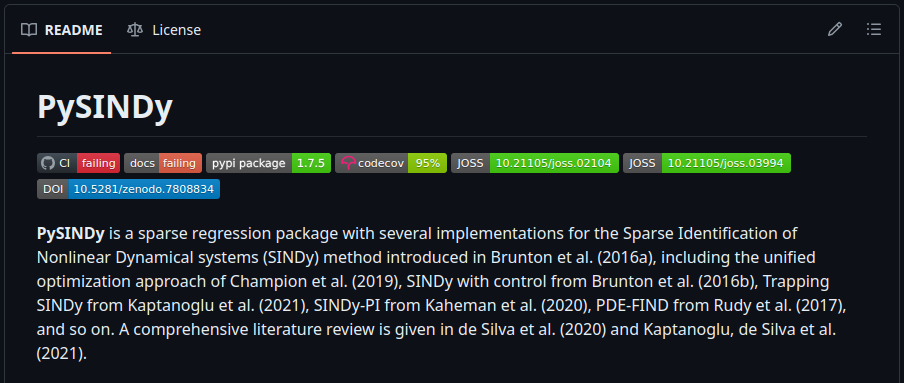
\includegraphics[width=\textwidth]{imgs/pysindy.png}
    \end{minipage}%
    \hfill
    \begin{minipage}{.58\textwidth}
        \begin{itemize}
            \item Open-source \texttt{Python} package with a simple and \texttt{scikit-learn} compatible API.
            \par\bigskip
            \item We're always on the look for new contributors!
            \begin{itemize}
                \item More computationally efficient algorithms.
                \item New/better variants of \textbf{SINDy}.
            \end{itemize}
        \end{itemize}
    \end{minipage}
    \vfill
\end{frame}

% \begin{frame}
%       \frametitle{A frame with title and subtitle}
%       \framesubtitle{Subtitle here}
%       Lorem ipsum dolor sit amet, consectetur adipiscing elit, sed do eiusmod tempor incididunt ut labore et dolore magna aliqua \par
%       Itemized list:
%       \begin{itemize}
%             \item Lorem ipsum
%             \item Dolor sit amet
%                   \begin{itemize}
%                         \item Consectetur
%                         \item Adipiscing elit
%                   \end{itemize}
%             \item Sed do eiusmod
%                   \begin{itemize}
%                         \item Tempor incididunt
%                               \begin{itemize}
%                                     \item Ut labore et dolore
%                                     \item Magna aliqua
%                               \end{itemize}
%                   \end{itemize}
%       \end{itemize}
% \end{frame}

% \begin{frame}
%       \frametitle{A frame with title only}
%       \begin{theorem}
%             \[e^{i\pi}+1=0\]
%             \begin{proof}
%                   \begin{equation*}
%                         e^{iz}=\cos{z}+i\sin{z}
%                   \end{equation*}
%                   \center{therefore}
%                   \begin{align*}
%                         e^{i\pi}+1 & \null=\cos\pi+i\sin\pi+1 \\
%                                    & \null=-1+i\times0+1      \\
%                                    & \null=0
%                   \end{align*}
%             \end{proof}
%       \end{theorem}
% \end{frame}

% \begin{frame}[bg=demo-arguelles.png]
%       \frametitle{A frame with background image}
%       You can still add title and subtitle. \par
%       You can also use a background in the title slide by setting: \\
%       \texttt{\textbackslash frame[plain,bg=demo-background.jpg]\{\textbackslash titlepage\}}
% \end{frame}

% \begin{frame}[plain]
%       \frametitle{A plain frame has no headline}
%       \begin{table}
%             \small
%             \begin{tabular}{rl}
%                   \ttfamily\textbackslash Alegreya              & \Alegreya Lorem ipsum dolor sit amet              \\
%                   \ttfamily\textbackslash AlegreyaMedium        & \AlegreyaMedium Lorem ipsum dolor sit amet        \\
%                   \ttfamily\textbackslash AlegreyaExtraBold     & \AlegreyaExtraBold Lorem ipsum dolor sit amet     \\
%                   \ttfamily\textbackslash AlegreyaBlack         & \AlegreyaBlack Lorem ipsum dolor sit amet         \\
%                   \ttfamily\textbackslash AlegreyaSansThin      & \AlegreyaSansThin Lorem ipsum dolor sit amet      \\
%                   \ttfamily\textbackslash AlegreyaSansLight     & \AlegreyaSansLight Lorem ipsum dolor sit amet     \\
%                   \ttfamily\textbackslash AlegreyaSans          & \AlegreyaSans Lorem ipsum dolor sit amet          \\
%                   \ttfamily\textbackslash AlegreyaSansMedium    & \AlegreyaSansMedium Lorem ipsum dolor sit amet    \\
%                   \ttfamily\textbackslash AlegreyaSansExtraBold & \AlegreyaSansExtraBold Lorem ipsum dolor sit amet \\
%                   \ttfamily\textbackslash AlegreyaSansBlack     & \AlegreyaSansBlack Lorem ipsum dolor sit amet
%             \end{tabular}
%       \end{table}
%       \vfill
%       \begin{alert}{Alert!}
%             A \textit{plain} frame does not show the progress bar but still appears in it unless the frame comes after \texttt{\textbackslash End}
%       \end{alert}
% \end{frame}

% \begin{frame}[standout]
%       \centering\large
%       A \textbf{\itshape\scshape standout} frame can be used to focus attention
% \end{frame}

\End

\begin{frame}
    This presentation wouldn't have been possible without many collaborators, including (but not limited to): 
    
    Steven Brunton, Bing Brunton, Nathan Kutz, Jared Callaham, Kathleen Champion, Brian da Silva, Alan Kaptanoglu, Kadierdan Kaheman, Urban Fasel, Sam Rudy, Zachary Nicolaou, Georgios Rigas, Nicholas Zolman and many others.
\end{frame}

\begin{frame}[plain,standout]
    \vfill
    \begin{minipage}{.68\textwidth}
        {
        \Large
        \textbf{Thank you for your attention!}
        }
        \par\bigskip
        {
        Any questions?
        }
    \end{minipage}%
    \hfill
    \begin{minipage}{.28\textwidth}
        \centering
        \scalebox{4}{\faGithub} \par\bigskip
        \tiny
        \url{loiseaujc.github.io}
        \par\medskip
        \url{github.com/dynamicslab/pysindy}
    \end{minipage}
    \vfill
    \end{frame}

\end{document}
